\section{Evaluation}

We implemented a prototype of the system with the aim of evaluating its efficacy along
a few different dimensions. First, we use metrics and a held-out data set to evaluate the quality
of the recommendation, i.e., how well the system selects valid follow-up questions for incomplete bug reports.
Second, we use a survey of software developers to evaluate the follow-up questions on their usefulness, novelty and specificity.


\subsection{Quality of Follow-Up Question Ranking}

One way of evaluating the ranking system, based on a held-out dataset (of bug reports and candidate follow-up questions), is
by using the posed questions as the ground truth. However, this simple setup has a serious deficiency in that the posed question
may not always be the most optimal among the set of candidate follow-up questions. More importantly, several of
the remaining candidate questions may be valid and (more) relevant to the bug report and therefore should
not be considered as negatively labeled instances for evaluation. Therefore, in order to provide an evaluation
set that identifies all of the valid questions in the candidate set, we perform manual annotation that clearly
identifies all of the valid follow-up questions for a specific bug report.

\subsubsection{Annotation}
We annotated 400 randomly chosen bug reports that were held out from our original corpus of 25K. The annotation
was performed by two of the authors following an agreed-upon predefined procedure. For each bug report, each annotator 1)
read the bug report carefully, spending a few minutes to understand its context, e.g., by looking at the purpose of the overall GitHub
project and the types of technologies it relies on; 2) marked all of the follow-up questions for the candidate set of 10
that were valid. Both of the annotators processed the same set of 400 bug reports, marking an average of 3.45/10 of the follow up questions as valid with an inter-annotator agreement (Cohen's kappa) of 0.60.
We use the set of follow-up questions that both annotators agreed were valid, i.e., the intersection between their annotation.

\subsubsection{Baselines}
The baselines we identified are meant to convey both straightforward approaches to ranking (e.g., directly using the Lucene output) and
ablation, i.e., using one part of our ranking function but not the other (e.g., ranking based only on the question utility, $U(q_{i})$).
We did not find appropriate prior research work to compare against, since the research direction is novel and models from other domains
with a similar purpose are too different in form. Below is an enumerated list of all of the ranking baselines we used.
\begin{itemize}
\item {\em Random} -- A random permutation of the candidate follow-up question list. We present metrics averaged over 10 runs.
\item {\em Lucene} -- Lucene uses the vector space model (i.e., tf*idf) to rank follow-up questions based on the similarity between the bug reports. This baseline just transfers Lucene's ranking, which we use to generate our candidate set of 10 follow-up questions, as the system's output.
\item {\em Utility only} -- $U(q_{i})$ -- The utility function, described in detail in Section~\ref{sec:ranking}, computes the average amount of OB,EB or S2R found in the answers to the specific follow-up question.
\item {\em Compatibility only} -- $P(q_{i}+a_{i}|br)$ -- The compatibility function computes the probability a bug report can be combined with a specific follow-up question and answer pair. The implementation uses a deep NN architecture to compute this quantity.
\end{itemize}

\subsubsection{Metrics}
We use a two popular information retrieval evaluation metrics: Mean Reciprocal Rank (MRR) and Precision@n (P@n).

The goal of MRR is to evaluate how effective is our technique, or a baseline, in locating the first valid follow-up question, as, presumably, this is a proxy for the ease with which an end-user would locate a follow-up question in the ranking. It is
computed as: $$MRR = \frac{1}{|B|} \sum_{i=1}^{|B|} \frac{1}{rank_{i}}$$ ,where $B$ is the set of bug reports in the test set and $rank_{i}$ is the ranked position of the first valid follow-up question for the $i^{th}$ bug report.

The goal of Precision@n is to measure the number of valid results when considering the top $n$ positions in the ranking. Unlike MRR, it consider all, not only the topmost ranked, results. It is computed as: $$P@n = \frac{1}{|B|} \sum_{i=1}^{|B|} \frac{|v|}{n}$$ ,where, as before, $B$ is the set of bug reports in the test set and $v$ is the set of valid follow-up questions ranked in the top $n$ positions. We use values of 1, 3 and 5 for $n$.


\begin{table}[t]
\centering
\caption{Evaluation results contrasting our system (\evpi) relative to several baselines.}
\begin{tabular}{p{3cm}cccc}
\hline
%                          & \multicolumn{4}{c}{$V_{1} \cap V_{2}$} \\\hline
                          & {\bf MRR}  & {\bf P@1}  & {\bf P@3}  & {\bf P@5}  \\\hline
{\em Random}              & 0.52 & 0.32 & 0.33 & 0.34 \\
{\em Lucene}              & 0.53 & 0.35 & 0.32 & 0.32 \\
{\em Utility only}        & 0.65 & 0.47 & 0.44 & 0.41 \\
{\em Compatibility only}  & 0.61 & 0.43 & 0.38 & 0.38 \\
{\em \evpi}                & 0.67 & 0.49 & 0.49 & 0.45 \\ \hline
\end{tabular}
\label{tab:results}
\end{table}


\subsubsection{Results} We summarize the results of our technique (\evpi) versus the identified
baselines in Table~\ref{tab:results}. Our results indicate that \evpi outperforms all of the baselines,
with the ablation-type baselines performing better than the simple baselines. The Lucene ranking
does surprisingly poor, basically in line with the Random baseline. The Utility only baseline is
the ones that comes closest to the performance of the full system. Perhaps the most intuitive result
is $P@1$, where \evpi scores 0.49, indicating that just about half of all of the top selected follow-up
questions by our system were valid.


\subsection{Developer Survey}
While a recommended follow-up question may be valid, it may not possess other properties that would
encourage its use in practice, i.e., in a system that automatically poses follow-up questions for incomplete bug reports. For
instance, a follow-up question may be overly generic, lacking detail or context specific to the bug report (e.g., {\em Can you provide
additional information?}). To investigate how \evpi performs across several such dimensions of interest we conducted a survey with
software developers.

%\subsubsection{Participants}
Through personal contacts, we e-mailed 10 software developers about the study, providing the basic context of our project
and a link to a Web form containing the survey. None of the developers were
aware about the details of our technique. The developers were half (5) from academia (graduate students at
institutions in the U.S. and Europe) and half professional developers from industry. All had programming
experience of 4 or more years with popular languages like Java and Python and all indicated one of their primary
responsibilities was developing software.

%Procedure
We randomly assigned the developers into two groups of 5 and each group was assigned 12 instances of bug report and follow-up question pairs, where all of the follow-up questions were the top-1 selected by \evpi. Each group was presented with bug reports from our corpus that belong to GitHub projects where Java or Python were the primary technologies used. For each one of the assigned bug reports, a developer
was presented with a screenshot from GitHub containing the title and text of the bug report, the follow-up question, and a link to the project the bug report came from for context. Prior to beginning the survey, we gave instructions to the developers to read both the bug report and the follow-up question before answering the provided set of survey questions. A preliminary survey question, which was posed on an initial screen, asked {\em Is the follow-up question valid?}. A negative response indicated that the follow-up question was invalid and unusable, so, therefore we asked no additional survey questions for that specific bug report - follow-up question pair. The remaining survey questions only appeared for instances deemed valid by a developer.

%Measures
For a valid follow-up question, we posed a yes/no survey question interrogating {\em Does the follow-up question ask for new information currently not included in the description?}, followed by two Likert score survey questions (5 point; Strongly Disagree, Disagree, Neutral, Agree, Strongly Agree) interrogating {\em The follow-up question is specific to the bug report} and {\em The follow-up question is useful to the bug report}. In the following, we refer to the first (yes/no) survey question as measuring New Information, the second measuring Specificity, and the third measuring Usefulness.

\begin{table}[t]
\centering
\caption{Inter-rater agreement for developer survey.}
\begin{tabular}{p{3cm}c}
\hline
                          & {\bf Fleiss' Kappa}   \\\hline
{\em Validity}                & 0.00  \\
{\em New Information}         & 0.00  \\
{\em Specificity}             & 0.00  \\
{\em Usefulness}              & 0.00  \\ \hline
\end{tabular}
\label{tab:kappa}
\end{table}

\begin{figure*}[t]
\centering
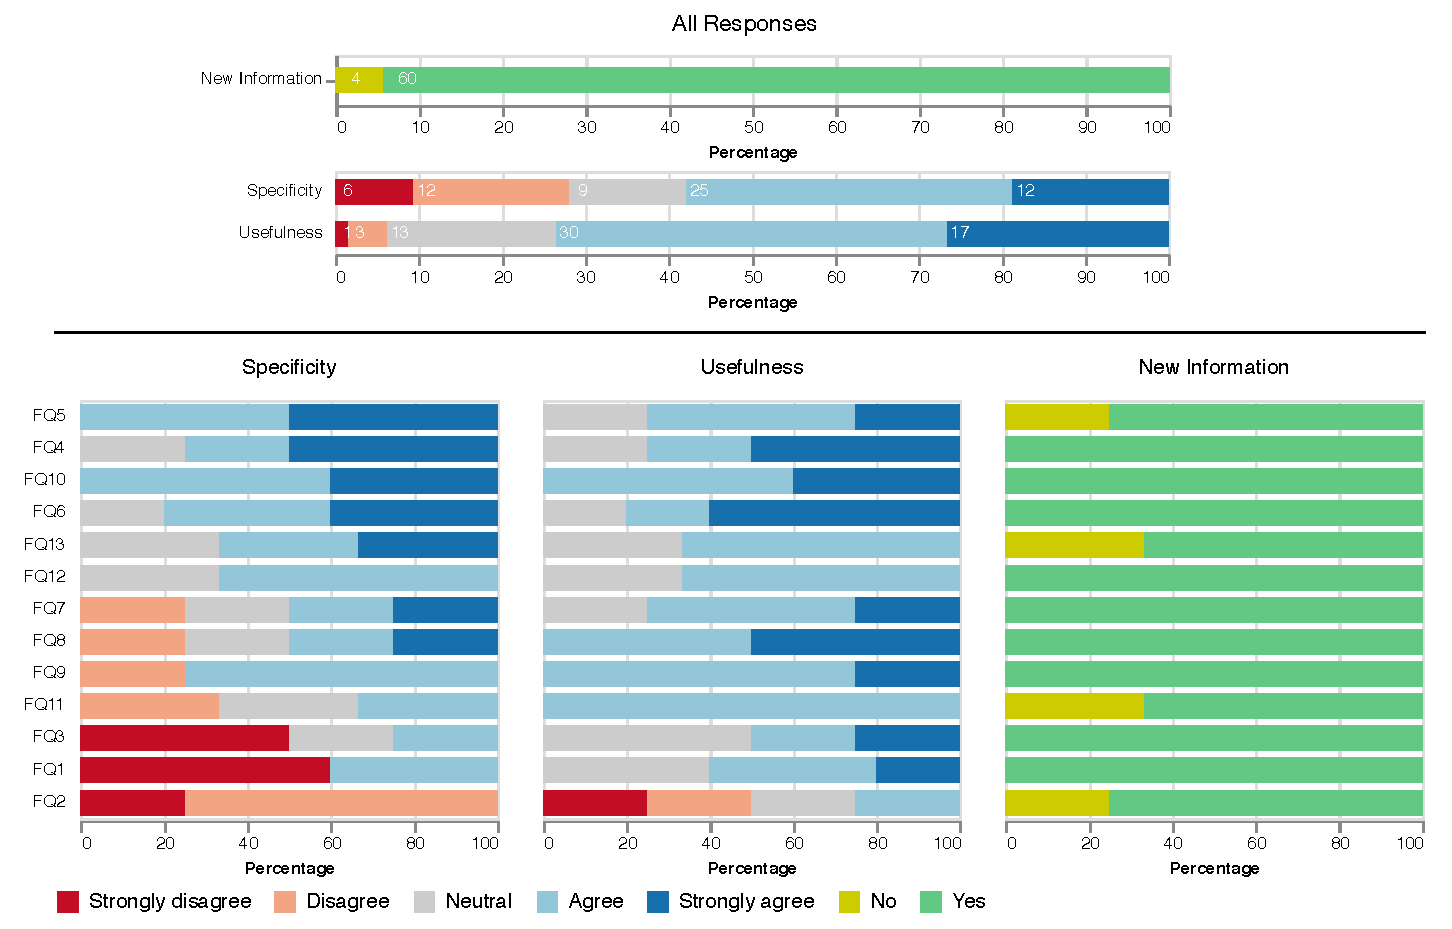
\includegraphics[width=0.99\linewidth]{figures/viz_group.pdf}
\caption{Responses to developer survey grouped per follow-up question (bottom) and per individual response (top).}
\label{fig:survey}
\end{figure*}

%Results
The survey results showed that out of the 24 different bug report - follow-up question pairs, a majority of participants (at least 3 out of 5) considered 13 follow-up questions as valid, and 11 as invalid. This ratio is analogous to the results we observed for Precision@1 in the held-out set evaluation above, confirming expectations.

The results of the survey, along each dimension, are presented both at the granularity of individual response in Figure X and at the granularity of a bug report (and follow-up question pair) in Figure Y. Figure X shows that ... In Figure Y we observe that
The inter-rater agreement, computed along each survey question, is shown in Table~\ref{tab:kappa}.



\subsection{Threats to Validity}
